\documentclass{beamer}
\usepackage{pgffor,pgfmath}
\usepackage{lipsum}
\usepackage{multicol}
\usetheme{ucla}
\usepackage{graphicx}
\usepackage{listings}
\usepackage{verbatim}
\usepackage{tikz}
\linespread{1.5}
\usepackage{comment}

\usepackage{amsmath, amsthm, amssymb, latexsym}

%\newtheorem{definition}{Definition}

\title{Lecture 7}
\author{Charles Rambo}
\institute{UCLA Anderson School of Management}
\date{2023}
\location{Los Angeles, California}

% Turn on slide numbers:
\showSlideNumber{}

\AtBeginSection[]
{
    \begin{frame}
        \frametitle{Table of Contents}
        \tableofcontents[currentsection]
    \end{frame}
}


\begin{document}

\insertTitleSlide

\section{Combinatorics}

\begin{frame}
\frametitle{Combinatorics}
\begin{Definition}
{\bf Combinatorics} is the branch of mathematics concerned with counting.
\end{Definition}
The fundamental counting principle states:
\begin{quote}
If there are $m_k$ ways to make the $k$-th decision for $k = 1, 2,\ldots n$, then there are a total of 
$$
\prod_{k = 1}^n m_k = m_1\cdot m_2\cdot\ldots\cdot m_n
$$ 
ways to make the $n$ independent decisions. 
\end{quote}
\end{frame}

\begin{frame}[t]
\frametitle{Combinatorics Example}
\small
\begin{Example}
Let's say that the personal code for your bank pin consists of six characters, each of which can be any letter or numerical digit.
\begin{enumerate}
\item[(a)] How many possible personal codes are there?
\item[(b)] Suppose you want your pin to have no repeated characters. How many possible pins would there be now?
\end{enumerate}
\end{Example}
\end{frame}

\subsection{Permutations and Combinations}

\begin{frame}
\frametitle{Permutations and Combinations}
\begin{Definition}
If the order in which the objects are chosen matters, each complete selection of $k$ objects from an original $n$ is called a {\bf permutation}. If the order does not matters, then each complete selection is called a {\bf combination}.
\end{Definition} 

\end{frame}

\begin{frame}
\frametitle{Permutations and Combinations without Repetition}

The number of permutations of $k$ elements from a selection of $n$ {\it without repetition} is 
$$
_n P_k = \frac{n!}{(n - k)!}.
$$
The number of combinations of $k$ elements from a selection of $n$ {\it without repetition} is 
$$
_nC_k = {n\choose k} =  \frac{n!}{k!(n-k)!}.
$$

\end{frame}

\begin{frame}[t]
\frametitle{Permutations and Combinations without Repetition}
\begin{Example}
\begin{enumerate}
\item[(a)] Among eight comparable investment funds, {\it ex ante}, how many different ways are there to list the top three performing funds?
\item[(b)] How may three-element subsets does a set containing nine elements have?
\end{enumerate}
\end{Example}
\end{frame}

\begin{frame}
\frametitle{$\boldsymbol n$ Elements of $\boldsymbol k$ Types}
Suppose there are $n_k$ indistinguishable elements of type $k$, where $k = 1, 2,\ldots m$. Let
$$
n = n_1 + n_2 + \ldots + n_m.
$$
Then the number of unique rearrangements of the $n$ elements is
$$
{n \choose n_1, n_2,\ldots, n_m} = \frac{n!}{n_1! n_2!\ldots n_m!}.
$$
\end{frame}

\begin{frame}[t]
\frametitle{$\boldsymbol n$ Elements of $\boldsymbol k$ Types}
\begin{Example}
How many unique rearrangements of the letters in BANANA are there?
\end{Example}
\end{frame}


\subsection{Stars-and-Bars}

\begin{frame}
\frametitle{Stars-and-Bars}

\begin{Theorem}[Stars-and-Bars]
Suppose there are $k$ types of items. If the order in which items are selected does not matter, the number of ways to select $n$ items is
$$
{n + k - 1\choose k - 1} = {n + k - 1\choose n}.
$$
\end{Theorem}
\end{frame}

\begin{frame}[t]
\frametitle{Stars-and-Bars Example}
\begin{Example}
In how many ways can we write the number 11 as the sum of five positive integers?
\end{Example}
\end{frame}

\begin{frame}
\frametitle{Stars-and-Bars on YouTube}
\small 
Watch Ken Ribet explain Stars-and-Bars (\url{https://youtu.be/UTCScjoPymA}).
\begin{center}
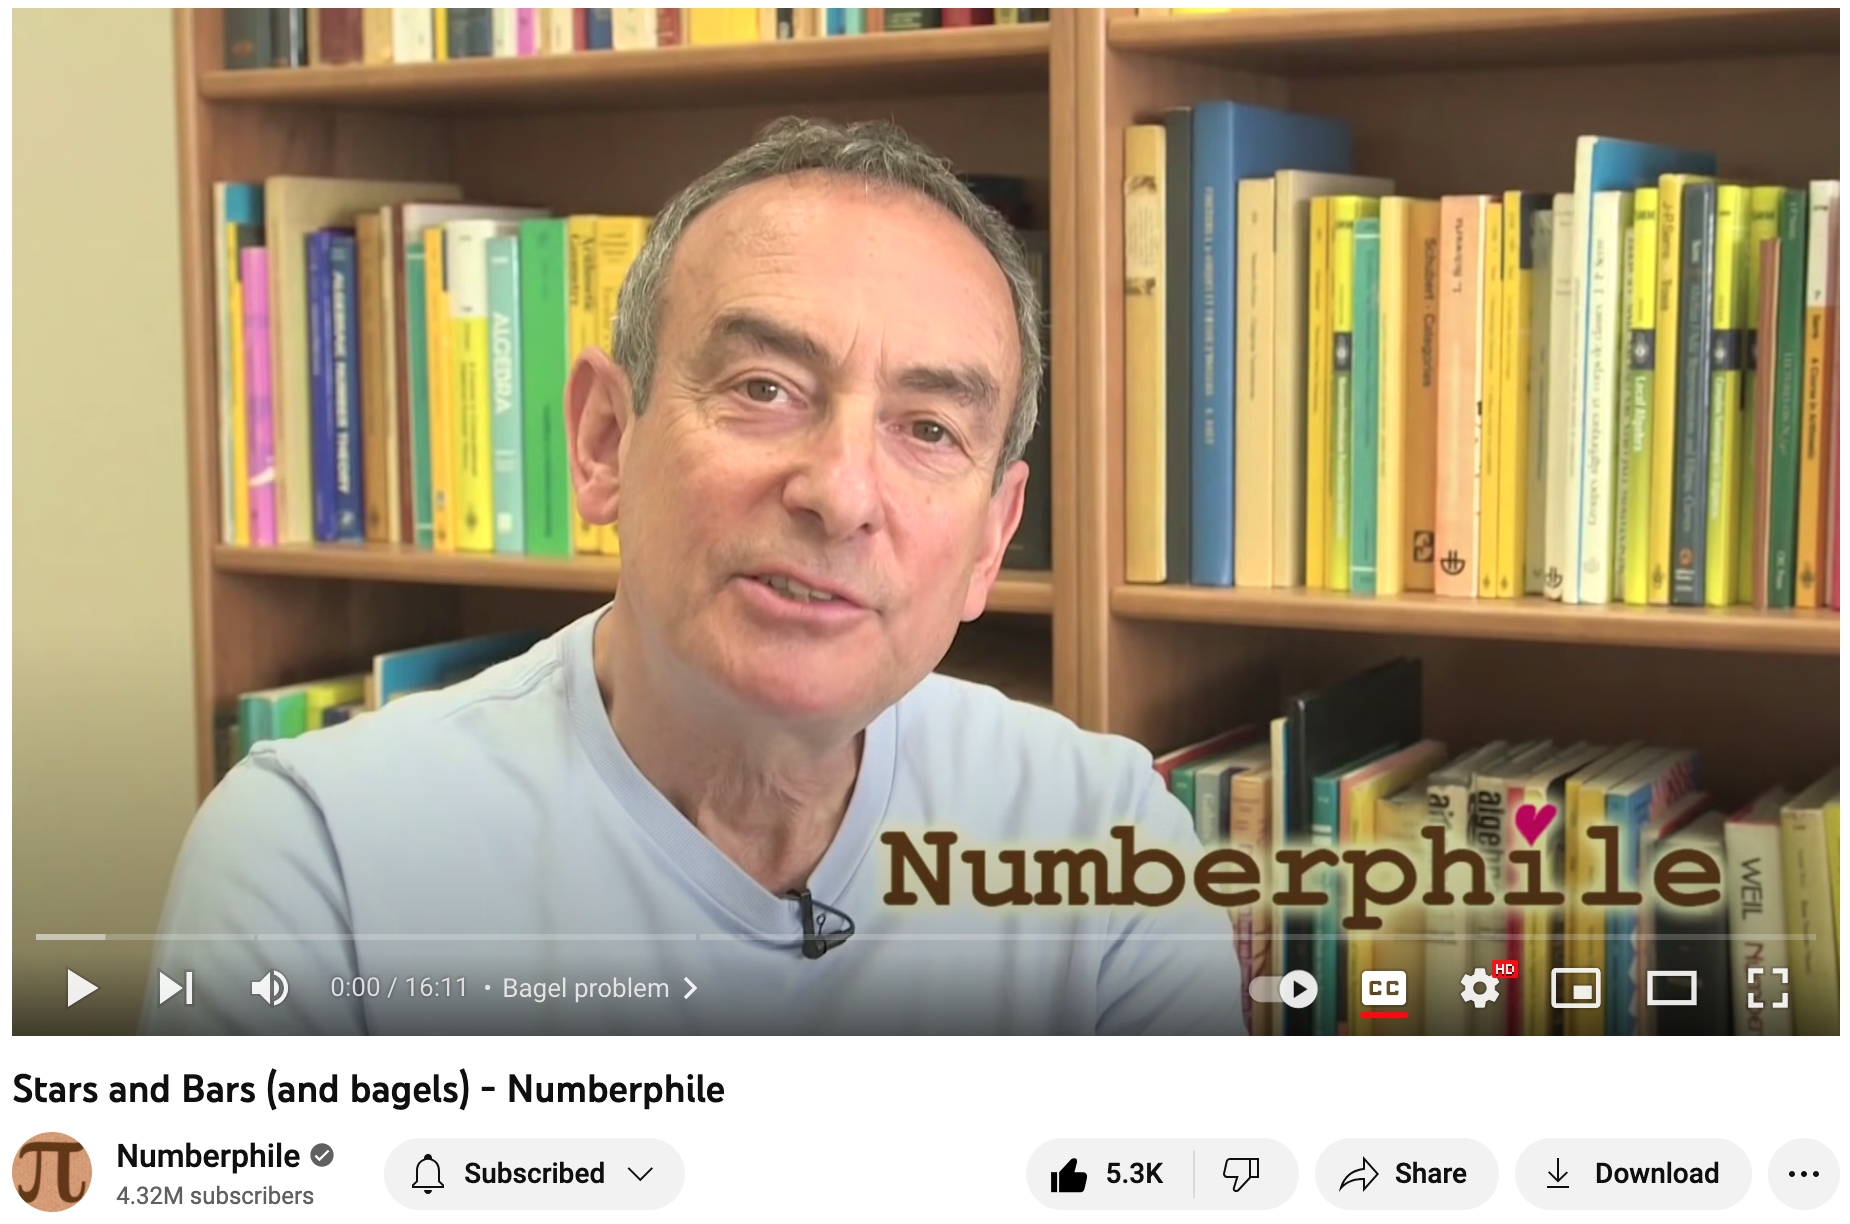
\includegraphics[scale = 0.25]{ribet.png}
\end{center}

\end{frame}

\subsection{The Pigeonhole Principle}

\begin{frame}
\frametitle{The Pigeonhole Principle}
Suppose there are $n$ objects distributed among $m$ sets, where $n \geq m$. Then one set must contain at lest $\lceil n/m \rceil$ elements.
\end{frame}

\begin{frame}[t]
\frametitle{The Pigeonhole Principle Example}
\begin{Example}
Suppose we have a set of $n + 1$ element. Show that we can always select two elements $a$ and $b$ such that $a - b$ is divisible by $n$.
\end{Example}

\end{frame}

\subsection{Inclusion--Exclusion Principle}

\begin{frame}
\frametitle{Inclusion--Exclusion Principle}
Suppose $|A|$ denotes the number of elements in $A$. Consider finite sets $A_1$ and $A_2$. The number of elements in $A_1\cup A_2$ is
$$
|A_1\cup A_2| = |A_1| + |A_2| - |A_1\cap A_2|.
$$
More generally, for $A_1, A_2,\ldots A_n$, the number of elements in $\displaystyle\bigcup_{i = 1}^n A_i$ is
\begin{align*}
\left|\bigcup_{i = 1}^n A_i\right| &= \sum_{i = 1}^n |A_i| - \sum_{1 \leq i < j \leq n} \left|A_i\cap A_j \right|+ \sum_{1\leq i < j < k\leq n} \left| A_i \cap A_j \cap A_k\right|\\
						&\qquad  - \ldots + (-1)^{n +1} \left|A_1\cap A_2\cap \ldots \cap A_n\right|.
\end{align*}

\end{frame}

\begin{frame}[t]
\frametitle{Inclusion--Exclusion Principle Example}
\tiny
\begin{Example}
There are 75 students enrolled in the class of 2024. Forty students are taking statistical arbitrage, 34 are taking credit markets, and 35 are taking behavioral finance. If fifteen students are taking statistical arbitrage and credit markets, 10 are taking statistical arbitrage and behavioral finance, and 17 are taking credit markets and behavioral finance, how many students are taking all three classes?
\end{Example}
\end{frame}

\section{Probability}

\begin{frame}
\frametitle{$\boldsymbol\sigma$-Algebra}
\begin{Definition}
Let $\Omega$ be some set, and let $2^\Omega$ represent the set of all subsets of $\Omega$. Then a subset $\mathcal{F}$ of $2^\Omega$ is called a $\boldsymbol\sigma$-{\bf algebra} if and only if it satisfies the following three properties:
\medskip

\begin{quote}
\begin{enumerate}
\item[SA.1] $\Omega$ is in $\mathcal{F}$.
\item[SA.2] If $A\in \mathcal{F}$ then $A^c = \{x\in\Omega: x\not\in A\}  \in\mathcal{F}$.
\item[SA.3] If $A_k\in\mathcal{F}$ for $k = 1, 2,\ldots$, then $\displaystyle\bigcup_{k= 1}^\infty A_k\in\mathcal{F}$.
\end{enumerate}
\end{quote}
\end{Definition}
\end{frame}

\begin{frame}
\frametitle{Probability Definition}
\begin{Definition}
Let $\Omega$ be a set and let $\mathcal{F}$  be a $\sigma$-algebra of $\Omega$. A {\bf probability} is defined as a function $P:\mathcal{F}\to [0, 1]$ if the following hold:
\medskip

\begin{quote}
\begin{enumerate}
\item[P.1] $P(\varnothing) = 0$.
\item[P.2] $P(\Omega) = 1$.
\item[P.2] For $E_k \in\mathcal{F}$ and $E_k\cap E_\ell= \varnothing$ for $k\neq \ell$, we have
$$
P\left(\bigcup_{k = 1}^\infty E_k\right) = \sum_{k = 1}^\infty P(E_k).
$$
\end{enumerate}
\end{quote}
We typically call $\Omega$ the {\bf sample space}. The elements of $\mathcal{F}$ are called {\bf events}. Altogether, $(\Omega, \mathcal{F}, P)$ forms a {\bf probability space}.
\end{Definition}
\end{frame}

\begin{frame}
\frametitle{Probability Example}
\begin{Example}
Consider the sample space $[0, 1]\times [0, 1]$. We define $P:\mathcal{F}\to [0, 1]$ such that $P(E) = \text{area}(E)$. In this cases, we would have 
$$
\mathcal{F} = \{E \subseteq [0, 1]\times [0, 1]: \text{area of}\ E\ \text{exists}\}.
$$
We need $\mathcal{F}$ because there are subsets of $[0, 1]\times [0, 1]$ whose area can't be measured!
\end{Example}
\end{frame}

\begin{frame}
\frametitle{Properties of Probability Measure}
Consider the probability space $(\Omega, \mathcal{F}, P)$. Suppose $A$ and $B$ are in $\mathcal{F}$.
\begin{itemize}
\item $A \subseteq B$ implies $P(A) \leq P(B)$
\item $P(A^c) = 1 - P(A)$
\item $P(A\cup B) = P(A) + P(B) - P(A\cap B)$
\end{itemize}
\end{frame}

\begin{frame}[t]
\frametitle{Probability Example}
\small
\begin{Example}
The point $(x, y)$ is selected at random from $[0, 1]\times [0, 1]$. Assume that all points within the sample space are equally likely to be selected. What is the probability that $xy$ is less than 1/2?
\end{Example}


\end{frame}

\subsection{Conditional Probability}

\begin{frame}
\frametitle{Conditional Probability}
\begin{Definition}
If the occurrence of the event $A$ depends on the occurrence of $B$ then the conditional probability is
$$
P(A | B) = \frac{P(A\cap B)}{P(B)}
$$
whenever $P(B) > 0$. If $P(B) = 0$ the conditional probability is undefined.
\end{Definition}

\end{frame}

\begin{frame}[t]
\frametitle{Conditional Probability Example}
\begin{Example}
Two fair dice are rolled. What is the probability that the sum of the dice are less than eight given that that the sum is even? 
\end{Example}
\end{frame}

\begin{frame}
\frametitle{Bayes' Rule}

\begin{Theorem}[Bayes]
Suppose $P(B) > 0$. Then
$$
P(A|B) = \frac{P(B|A) P(A)}{P(B)}.
$$
\end{Theorem}

\begin{Theorem}[Law of Total Probabilities]
Suppose $B_i \cap B_j = \varnothing$ for $i\neq j$ and $\displaystyle\bigcup_{i = 1}^n B_i = \Omega$. Then
$$
P(A) = P(A|B_1) P(B_1) + P(A|B_2)P(B_2) + \ldots + P(A|B_n) P(B_n).
$$
\end{Theorem}

\end{frame}

\begin{frame}[t]
\frametitle{Bayes' Rule Example}
\small
\begin{Example}
Suppose the probability that an unskilled asset manager beats the market is 50\%, and the probability that a skilled asset manager beats the market is 60\%. If 10\% of asset managers are skilled, what is the probability that an asset manager is skilled given that she beats the market?
\end{Example}

\end{frame}

\begin{frame}
\frametitle{Bayes' Rule on YouTube}
Watch the StatQuest video about Bayes' theorem (a.k.a. Bayes' rule) on YouTube (\url{https://youtu.be/9wCnvr7Xw4E}).
\begin{center}
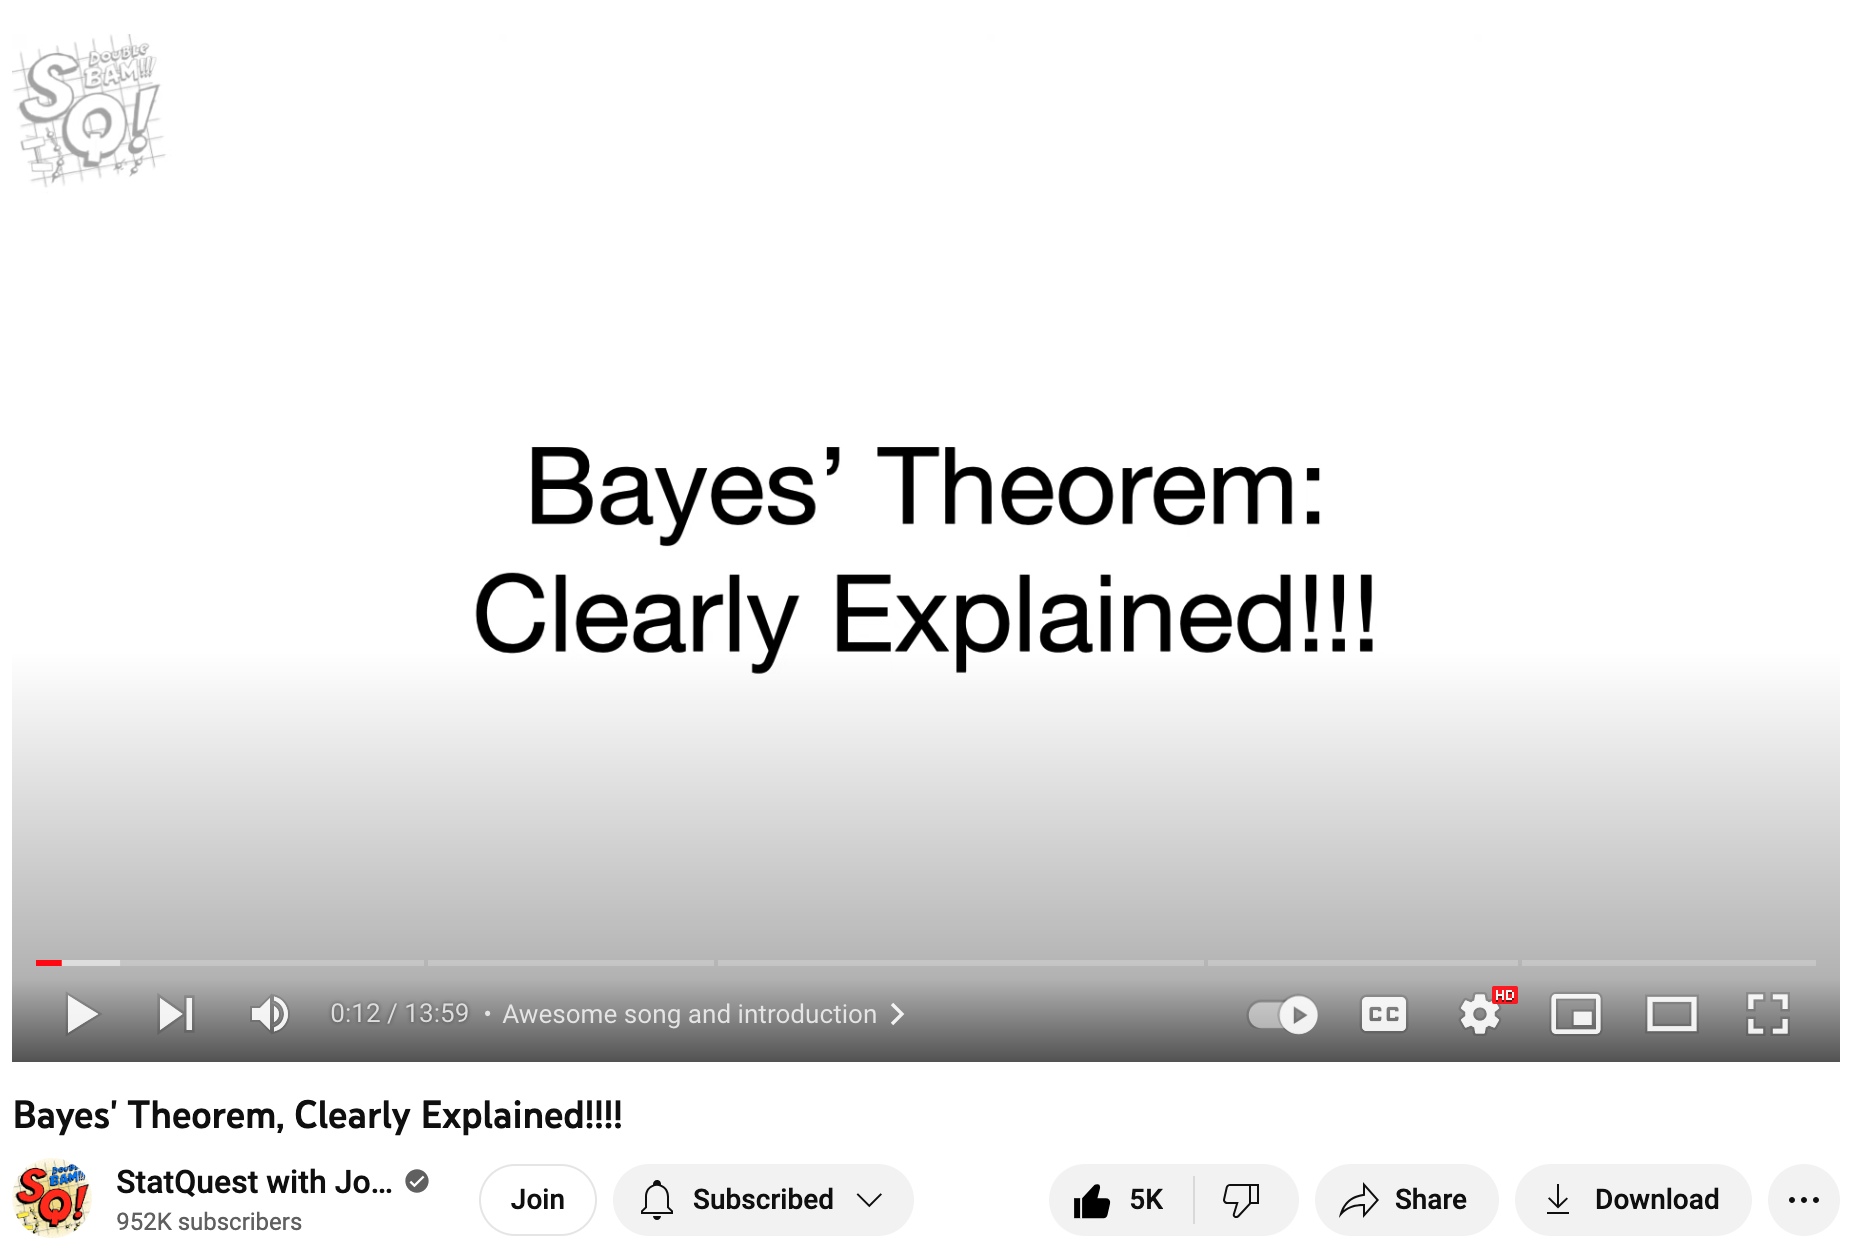
\includegraphics[scale = 0.25]{bayes_statquest.png}
\end{center}

\end{frame}

\begin{frame}
\frametitle{Independent Events}

\begin{Definition}
Events $A$ and $B$ are independent if $P(A|B) = P(A)$.
\end{Definition}
If two events are independent then it's easy to prove
$$
P(A\cap B) = P(A) P(B).
$$
\end{frame}

\begin{frame}[t]
\frametitle{Independent Events Example}
\small
\begin{Example}
One urn contains four red balls and six blue balls. A second urn contains sixteen red balls and $x$ blue balls. A single ball is drawn from each urn. The probability that both balls are the same color is 0.44 . Calculate $x$.
\end{Example}

\end{frame}

\subsection{Random Variables} 

\begin{frame}
\frametitle{Random Variables}

\begin{Definition}
A random variable $X$ is a function $X:\Omega\to\mathbb{R}$ where $P\left(X^{-1}(A)\right)$ exists for $A\subseteq\mathbb{R}$.
\end{Definition}

The probability that $X$ takes on values in the subset $S$ of $\mathbb{R}$ is written
$$
P(X\in S) = P\left(\{\omega \in\Omega : X(\omega)\in S\}\right).
$$
The probability that $X$ takes on value $x$ in $\mathbb{R}$ is written
$$
P(X = x) = P\left( \{\omega \in\Omega : X(\omega) = x\} \right).
$$
\end{frame}

\begin{frame}
\frametitle{Types of Random Variables}
There are three types of random variables: {\it discrete} random variables, {\it continuous} random variables, and {\it mixed} random variables. 
\begin{itemize}
\item A discrete random variable is a random variable whose range is either finite or countably infinite. 
\item A continuous random variable is a random variable whose range is an interval in $\mathbb{R}$. 
\item A mixed random variable is partially discrete and partially continuous.
\end{itemize}

\end{frame}

\begin{frame}[t]
\begin{Example}
State whether the random variables are discrete, continuous, or mixed.
\begin{enumerate}
\item[(a)] A coin is tossed ten times. The random variable $X$ is the number of tails.
\item[(b)] The random variable $Y$ measures the number of years until a firm defaults on its debt.
\item[(c)] $Z(X) = \begin{cases} 1 - X, &0\leq X < 1/2\\ 1, 	&1/2\leq X \leq 1\end{cases}$
where $X$ is a continuous random variables with range $[0, 1]$.
\end{enumerate}
\end{Example}

\end{frame}

\subsection{Discrete Random Variable}

\begin{frame}
\frametitle{Probability Mass Function}
\begin{Definition}
For a discrete random variable $X$, we define the {\bf probability mass function} or {\bf pmf} by the equation
$$
p(x) = P(X = x).
$$
\end{Definition}
\end{frame}

\begin{frame}[t]
\frametitle{Probability Mass Function Example}
\begin{Example}
A coin is flipped three times. Let the random variable $X$ denote the number of heads. Find the pmf of $X$.
\end{Example}

\end{frame}

\begin{frame}
\frametitle{Cumulative Distribution Function}
\begin{Definition}
For a discrete random variable $X$, we define the {\bf cumulative distribution} or {\bf cdf} by the equation
$$
F(x) = P(X\leq x) = \sum_{t \leq x} P(X = t).
$$
\end{Definition}
\end{frame}

\begin{frame}[t]
\frametitle{Probability Mass Function Example}
\begin{Example}
The random variable $X$ denotes the number selected from the set $\{1, 2, 3, 4\}$. If each number is equally likely, find the cdf.
\end{Example}

\end{frame}

\begin{frame}
\frametitle{Uniform Distribution}
\begin{Definition}
The {\bf discrete uniform distribution} is a symmetric probability distribution. In this distribution, a finite number of values are equally likely to be observed. Every one of the $n$ values has equal probability $1/n$ of being observed.
\end{Definition}
\end{frame}

\begin{frame}
\frametitle{Binomial Distribution}
\small 
\begin{Definition}
The {\bf binomial distribution} with parameters $n$ and $p$ is the discrete probability distribution of the number of successes in a sequence of $n$ independent experiments, each ending in either success with probability $p$ or failure with probability $q = 1- p$.
\end{Definition}
To denote that $X$ is a binomial random variable with parameters $n$ and $p$, we write $X\sim{\mathcal{B}(n, p)}$. The probability 
$$
\displaystyle P(X = x) = \begin{cases}{n\choose x} p^x q^{n - x},	&	x = 0, 1, \ldots, n\\ 0,	&\text{otherwise.}\end{cases}
$$
\end{frame}

\begin{frame}[t]
\frametitle{Binomial Distribution Example}
\small
\begin{Example}
Suppose a portfolio manager has a portfolio of 25 high yield bonds. She assumes that each bond has a one-year default probability of 5\%. Her portfolio is well diversified so defaults are independent. What is the probability that more than one bond defaults?
\end{Example}
\end{frame}

\begin{frame}[fragile]
\frametitle{Binomial Distribution Python Example}
\begin{Example}
Use Python to check the previous result by simulating the event 10,000 times. 
\end{Example}

{
\linespread{0.8}
{\bf Solution.}  
{\tiny
\begin{verbatim*}
import numpy as np
from scipy.stats import binom

# Generate 10,000 simulations
defaults = binom.rvs(n = 25, p = 0.05, loc = 0, size = 10000, random_state = 0)

# Calculate probability
prob = np.mean(defaults > 1)

print(f'The probability that more than one bond defaults is {prob:.3f}.')
\end{verbatim*}
}}
The output is 0.351.

\end{frame}

\begin{frame}
\frametitle{Poisson Distribution}
\begin{Definition} 
The {\bf Poisson distribution} is a discrete probability distribution that expresses the probability of a given number of events $x$ occurring in a fixed interval if these events occur independently with a constant rate $\lambda$.
\end{Definition}
To denote that $X$ is a Poisson random variable with parameter $\lambda$, we write $X\sim{\mathcal{P}(\lambda)}$. The probability 
$$
P(X = x) = \begin{cases} \dfrac{\lambda^x e^{-\lambda}}{x!},&  x = 0, 1, 2,\ldots\\ 0,	&	\text{otherwise.}\end{cases}
$$
\end{frame}

\begin{frame}[t]
\frametitle{Poisson Distribution Example}
\tiny
\begin{Example}
After graduation from the MFE program, you become a successful and famous portfolio manager. To help younger men and women succeed in finance, you begin writing a memoir of your life. In the first draft of your book, there are an average of fifteen spelling errors per page. Suppose that the number of errors per page follows a Poisson distribution. What is the probability of having no errors on a page?
\end{Example}

\end{frame}


\subsection{Continuous Random Variable}



\end{document}